\documentclass{article}
\usepackage[utf8]{inputenc}
\usepackage{amsmath}
\usepackage{siunitx}
\usepackage{graphicx} 
\usepackage{float}
\usepackage{csquotes}
\usepackage[english]{babel}

\usepackage{biblatex}
\addbibresource{bibliography.bib}

\DeclareMathOperator*{\argmax}{arg\,max}

\title{Portfolio balancing with fractional set cover}
\author{Lucas Pettersson}
\date{July 2024}


\begin{document}

\maketitle
\newpage

\tableofcontents
\newpage

%%%%%%%%%%%%%%%%%%%%%%%%%%%%%%%%%%%%%
%%%%%%%%%%%%%%%%%%%%%%%%%%%%%%%%%%%%%
%%%%%%%%%%%%%%%%%%%%%%%%%%%%%%%%%%%%%
%%%%%%%%%%%%%%%%%%%%%%%%%%%%%%%%%%%%%

\addcontentsline{intro}{section}{Introduction}
\section{Introduction}
Trading with instruments including more than one asset often gives rise to the problem of homogeneity instead of a diverse portfolio. To solve this problem, the problem of fractional set covering is considered for balancing a portfolio. The set cover problem is as follows, given a set of vertices, $U$, and a collection of subsets of the vertices, find the minimum collection of subsets that covers $U$. Fractional set cover is a variant of the set cover problem where each set is allowed a continuous instead of a discrete selection for each vertice. \cite{bib:fracCover} 

\section{Problem statement}
Given a portfolio, $V$, with associated assets $v_i, \ldots, v_n$, and a collection of instruments, $V^* := \{V^*_1, \ldots, V^*_m$\}, with their own assets $v^*_{1,1}, \ldots, v^*_{1,k}$ such that $v_{i,j} \in V,~\forall i,j$. Find the minimal subset of $V^*$ that covers $V$.

\begin{figure}[H]
    \centering
    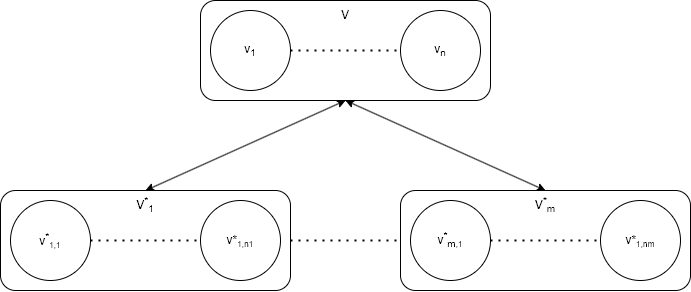
\includegraphics[scale=0.4]{figures/fracCov.png}
    \caption{Illustration of the fraction set cover problem.}
    \label{fig:fracCov}
\end{figure}

\noindent The assets can be defined as weights such that 

\begin{equation}
    \begin{cases}
        & 0 \leq v_i \leq 1 \\
        & \sum_i v_i = 1
    \end{cases}.
\end{equation}

\noindent Each instrument can be defined as a vector containing their own weights

\begin{equation}
    \begin{cases}
        & 0 \leq v^*_{i,k} \leq 1 \\
        & \sum_i v^*_{i,k} = 1
    \end{cases}.
\end{equation}

\noindent The problem is then to allocate each instrument such that weights of the instruments covers the portfolio. Let

\begin{equation}
    x := 
    \begin{pmatrix}
        x_1 \\
        \vdots \\
        x_m
    \end{pmatrix}
\end{equation}

\noindent be the selection of instruments such that 

\begin{equation}
    \sum_i x_i = 1,
\end{equation}

\noindent the weight vector for the portfolio

\begin{equation}
    b := 
    \begin{pmatrix}
        v_1 \\
        \vdots \\
        v_n
    \end{pmatrix},
\end{equation}

\noindent and the weight vectors for each instrument

\begin{equation}
    A^*_i := 
    \begin{pmatrix}
        v^*_{i,k} * I(v_1 \in V^*_i), ~ \arg_k \{ v_1 = v_{i,k} \}  \\
        \vdots \\
        v^*_{i,k} * I(v_n \in V^*_i), ~ \arg_k \{ v_n = v_{i,k} \}
    \end{pmatrix}.
\end{equation}

The problem can be formulated with linear programming such that

\begin{equation}
    \begin{split}
        \min_{x \in R^m} & 1^Tx \\
        s.t. & Ax \geq b
    \end{split}
\end{equation}

\noindent where $A$ is the matrix given by concatenating the weight vectors

\begin{equation}
    A:=
    \begin{pmatrix}
        A_1, \ldots, A_m
    \end{pmatrix}.
\end{equation}


\newpage
\section{References}
\printbibliography[heading=none]

\end{document}
